\documentclass[main.tex]{subfiles}

\begin{document}

\subsection{Secondo esercizio}

\begin{figure}[H]
\centering
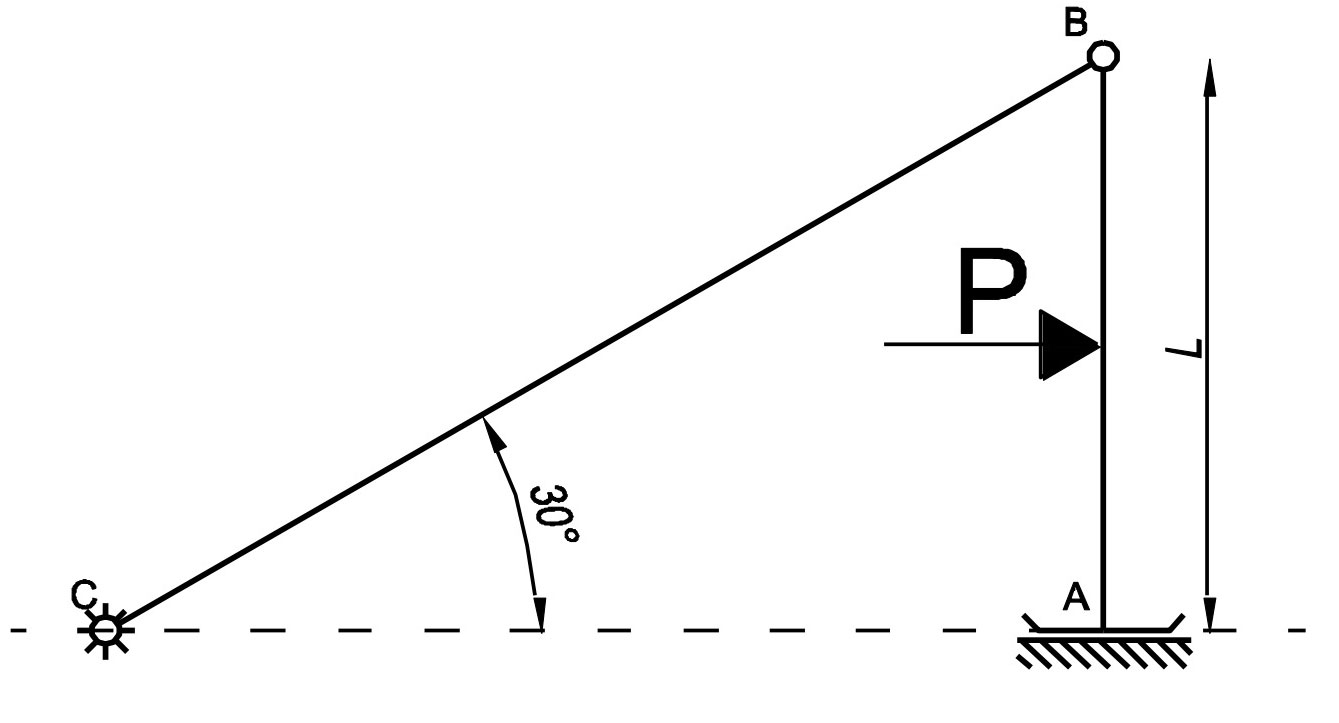
\includegraphics[width=0.75\textwidth]{2015-2602-2.jpg}
\end{figure}

La struttura in figura è soggetta alla sola forza orizzontale P.
\\
Si chiede di calcolare:
\begin{enumerate}
\item Le reazioni vincolari a terra (punti A e C).
\item Le azioni interne nell’asta AB (disegnare i corrispondenti diagrammi).
\end{enumerate}

\clearpage

\subsection{Soluzione secondo esercizio}

\subsubsection{Osservazioni}

\begin{enumerate}
\item La struttura è composta da un'asta AC, un pattino ed una biella CB.
\item La biella agisce inclinata di $30\deg$, per cui le componenti della reazione assiale saranno rispettivamente $\dfrac{2}{2}$ e $\dfrac{\sqrt{3}}{2}$ della reazione.
\end{enumerate}

\subsubsection{Analisi preliminare di isostaticità}
Verifico che $gdl_{tot} = gdv_{tot}$:
\begin{figure}[H]
  \begin{subfigure}[b]{.5\textwidth}
  \centering
  \[
  	gdv: \begin{cases}
		gdv_{pattino} = 2\\
		gdv_{biella} = 1
  	\end{cases}
  \]
  \caption{Gradi di vincolo del sistema.}
  \end{subfigure}
  \hfill
  \begin{subfigure}[b]{.5\textwidth}
  \centering
  \[
  	gdl: \begin{cases}
  		gdl_{asta} = 3\\
  	\end{cases}
  \]
  \caption{Gradi di libertà del sistema.}
  \end{subfigure}
  \caption{Verifica preliminare di isostaticità.}
\end{figure}

\subsubsection{Primo punto}

\paragraph{Analisi dei vincoli esterni}

\begin{figure}[H]
\centering
\resizebox{.5\textwidth}{!}{% First image 2015 06 29

\begin{tikzpicture}

  \tiny


  \point{c}{0}{0}
  \point{c1}{0}{0.8}
  \point{c2}{-0.8}{0}
  \point{a}{2-1.41421}{1.41421}
  \point{a1}{2-1.41421}{0.8+1.41421}
  \point{d}{2}{0}
  \point{b}{2+1.41421}{-1.41421}
  \point{b1}{2+1.41421}{-1.41421-1.3}

  \beam{2}{c}{d}[0][1];
  \beam{2}{a}{b};

  \load{1}{a}[180][0.5]
  \load{1}{a1}[270][0.5]

  \load{2}{c}
  \load{1}{c}[180][0.5]
  \load{1}{c}[270][0.5]

  \load{1}{b1}[90][1]

  \notation{1}{c}{$\vec{M}_C$}[below right]
  \notation{1}{c}{$\vec{H}_C$}[below left]
  \notation{1}{c}{$\vec{V}_C$}[above right]

  \notation{1}{a}{$\vec{H}_A$}[below left]
  \notation{1}{a}{$\vec{V}_A$}[above right]

  \notation{1}{b}{$\vec{F}$}[below right]

  % \notation{1}{a1}{$\vec{H}_A$}
  % % \notation{1}{d1}{$\vec{R}_D$}
  % % \notation{1}{b1}{$\vec{H}_B$}[below left]
  % \notation{1}{c1}{$\vec{F}$}[above left]

  %  % \support{3}{o};

  %  % %Degrees
  %  % \notation{1}{o}{$\alpha$}[above];
  %  % \notation{1}{a}{$\beta$}[above];

  %  % \notation{5}{o}{a}[$a$];
  %  % \notation{5}{a}{b}[$b$];
  %  % \notation{5}{o}{b}[$c$];

\end{tikzpicture}}
\caption{Analisi dei vincoli esterni}
\end{figure}

\[
\begin{cases}
	H_C = -P\\
	V_C = -V_A\\
	M_A + \dfrac{1}{2}LP + \sqrt{3}LV_C = 0
\end{cases}
\]

\paragraph{Analisi delle reazioni vincolari nell'asta CB}

\begin{figure}[H]
\centering
\resizebox{.5\textwidth}{!}{% First image 2015 06 29

\begin{tikzpicture}

  \tiny


  \point{c}{0}{0}
  \point{a}{1.73}{0}
  \point{b}{1.73}{1}
  \point{b1}{1.73}{0.5}

  \beam{2}{c}{b};

  \load{1}{c}[270][0.5]
  \load{1}{c}[180][0.5]

  \load{1}{b}[90][0.5]
  \load{1}{b}[0][0.5]

  \notation{1}{c}{$\vec{H}_C$}[below left]
  \notation{1}{c}{$\vec{V}_C$}[below right]

  \notation{1}{b}{$\vec{R}_{B_x}$}[below right]
  \notation{1}{b}{$\vec{R}_{B_y}$}[above left]

\end{tikzpicture}}
\caption{Reazioni vincolari nell'asta CB}
\end{figure}

\[
\begin{cases}
	H_C = R_{B_x} = -P\\
	V_C = R_{B_y}\\
	M_C = 0 = \sqrt{3}LR_{B_y} - LR_{B_x}\\
\end{cases}
\Longrightarrow
\begin{cases}
	H_C = R_{B_x} = -P\\
	V_C = R_{B_y}\\
	V_C = -\dfrac{\sqrt{3}}{3}P\\
\end{cases}
\]

Sostituisco nell'equazione di equilibrio dei momenti ed ottengo:

\[
	M_A + \dfrac{1}{2}LP - \sqrt{3}L\dfrac{\sqrt{3}}{3}P = 0
\]

\[
	M_A + \dfrac{1}{2}LP - LP = 0
\]

\[
	M_A  = \dfrac{1}{2}LP
\]

\paragraph{Riassumendo}

\begin{figure}[H]
  \begin{subfigure}[b]{.5\textwidth}
  \centering
  \[
  	A: \begin{cases}
		V_A = \dfrac{\sqrt{3}}{3}P\\
		M_A = \dfrac{1}{2}LP
  	\end{cases}
  \]
  \caption{Reazioni vincolari in A.}
  \end{subfigure}
  \hfill
  \begin{subfigure}[b]{.5\textwidth}
  \centering
  \[
  	C: \begin{cases}
  		V_C = -\dfrac{\sqrt{3}}{3}P\\\\
  		H_C = -P\\
  	\end{cases}
  \]
  \caption{Reazioni vincolari in C.}
  \end{subfigure}
\end{figure}


\subsubsection{Secondo punto}
Le componenti dei vettori, dato che l'asta AB è 	verticale, coincidono già con le componenti di sforzo normale e taglio.

\paragraph{Sforzo normale}
Lo sforzo normale è di contrazione e quindi è negativo.

\begin{figure}[H]
\centering
\resizebox{.25\textwidth}{!}{% First image 2015 06 29

\begin{tikzpicture}

  \tiny


  \point{c}{0}{0}
  \point{a}{0}{1}
  \point{b}{1}{0}
  \point{d}{2}{0}

   \beam{2}{c}{d}[0][1];

  \internalforces{c}{b}{1}{1}[0][blue];

\end{tikzpicture}}
\caption{Sforzo normale nell'asta AB}
\end{figure}

\paragraph{Taglio}
Nella tronco superiore, le forze $H_B$ e $P$ originano una rotazione \textbf{anti-oraria}, e creano quindi un taglio \textbf{negativo}. Nella tronco inferiore non è presente taglio.

\begin{figure}[H]
\centering
\resizebox{.25\textwidth}{!}{% First image 2015 06 29

\begin{tikzpicture}

  \tiny


  \point{c}{0}{0}
  \point{c1}{0}{0.8}
  \point{c2}{-0.8}{0}
  \point{a}{2-1.41421}{1.41421}
  \point{a1}{2-1.41421}{0.8+1.41421}
  \point{d}{2}{0}
  \point{d1}{2-0.8}{0}
  \point{b}{2+1.41421}{-1.41421}
  \point{b1}{2+1.41421}{-1.41421-1.3}

  \beam{2}{a}{b};

  \internalforces{a}{d}{-0.707}{-0.707}[0][blue];
  \internalforces{d}{b}{0.707}{0.707}[0][red];

\end{tikzpicture}}
\caption{Taglio nell'asta AB}
\end{figure}

\paragraph{Momento flettente}
Il momento flettente raggiunge il punto massimo nel punto di applicazione della forza $P$, dove vale $LP$. Successivamente si mantiene costante sino a raggiungere il punto A.
\\
\\
Le fibre tese si trovano sul lato di destra.

\begin{figure}[H]
\centering
\resizebox{.25\textwidth}{!}{% First image 2015 06 29

\begin{tikzpicture}

  \tiny


  \point{c}{0}{0}
  \point{c1}{0}{0.8}
  \point{c2}{-0.8}{0}
  \point{a}{2-1.41421}{1.41421}
  \point{a1}{2-1.41421}{0.8+1.41421}
  \point{d}{2}{0}
  \point{d1}{2-0.8}{0}
  \point{b}{2+1.41421}{-1.41421}
  \point{b1}{2+1.41421}{-1.41421-1.3}

  \beam{2}{a}{b};

  \internalforces{a}{d}{0}{-0.707}[0][red];
  \internalforces{d}{b}{-0.707}{0}[0][red];

\end{tikzpicture}}
\caption{Momento flettente nell'asta AB}
\end{figure}

\end{document}